\documentclass{beamer}
\usepackage{beamerthemesplit}
\usepackage{wrapfig}
\usetheme{SPbGU}
\usepackage{pdfpages}
\usepackage{amsmath}
\usepackage{cmap} 
\usepackage[T2A]{fontenc} 
\usepackage[utf8]{inputenc}
\usepackage[english,russian]{babel}
\usepackage{indentfirst}
\usepackage{amsmath}
\usepackage{tikz}
\usepackage{multirow}
\usepackage[noend]{algpseudocode}
\usepackage{algorithm}
\usepackage{algorithmicx}
\usetikzlibrary{shapes,arrows}
\usepackage{fancyvrb}
\newtheorem{rutheorem}{Теорема}
\newtheorem{ruproof}{Доказательство}
\newtheorem{rudefinition}{Определение}
\newtheorem{rulemma}{Лемма}
\beamertemplatenavigationsymbolsempty

\title[]{Разработка системы предсказания вторичной структуры РНК с использованием синтаксического анализа и искусственных нейронных сетей}
%\subtitle[]{Опциональный подзаголовок}
% То, что в квадратных скобках, отображается в левом нижнем углу. 
\institute[СПбГУ]{
Санкт-Петербургский государственный университет \\
Кафедра системного программирования }

% То, что в квадратных скобках, отображается в левом нижнем углу.
\author[Кутленков Дмитрий]{Кутленков Дмитрий Александрович, 371 группа(17.Б11-мм) \\
  % У научного руководителя должна быть указана научная степень
  \and  
    {\bfseries Научный руководитель:} к.ф.-м.н., доцент Григорьев С.В. \\ 
  % Для курсовой не обязателен. Должна быть указана должность или ученая степень
%  \and
%    {\bfseries Рецензент:} программист ООО ``Рога и копыта'' И.И. Иванов
}

\date{23 мая 2020г.}

\definecolor{orange}{RGB}{179,36,31}

\begin{document}
{
% Лого университета или организации, отображается в шапке титульного листа
\begin{frame}
  \begin{center}
  {
\includegraphics[width=1.5cm]{pictures/SPbGU_Logo.png}}
  \end{center}
  \titlepage
\end{frame}
}

\begin{frame}[fragile]
  \transwipe[direction=90]
  \frametitle{Введение}
  
%    \item Краткий обзор тематики работы (как вариант — устно, пока показывается титульный слайд)
%    \item Не нужно определять общеизвестные понятия
%    \item Применимость/полезность данной работы, обоснование выбора именно этой темы 
%    \item Если тема похожа на темы других работ (в том числе прошлых лет), надо явно описать разницу
\begin{tabular}{p{5cm} p{7cm}}
	\begin{itemize}
		\item РНК --- биологическая последовательность
		\item Ее первичная структура --- последовательность нуклеотидов, которые задаются алфавитом из 4 букв
		\item Вторичная структура --- то, как нуклеотиды образуют связи
  \end{itemize} &
%{\includegraphics[width=5cm]{../DNA_RNA_structure_(full).png}}
\multirow{-1.5}*{\!\includegraphics[width=4.5cm]{../pics/DNA_RNA_structure_(full).png}}
\end{tabular}

\end{frame}
            
\begin{frame}
  \transwipe[direction=90]
  \frametitle{Существующие решения}
  \begin{itemize}
  	\item Методы сравнительного анализа
    \item Метод минимальной свободной энергии (MFE) --- \textit{RNAfold}, \textit{CentroidFold}, \textit{HotKnots}, \textit{IPknot}
    \item Иерархическая свертка --- \textit{HFold}, \textit{Iterative HFold}
    \item Исследования с использованием машинного обучения
   
  \end{itemize}\medskip
   Не существует оптимального метода.

\end{frame}

% Обязательный слайд: четкая формулировка цели данной работы и постановка задачи
% Описание выносимых на защиту результатов, процесса или особенностей их достижения и т.д.
\begin{frame}
  \transwipe[direction=90]
  \frametitle{Постановка задачи}
  \textbf{Целью} данной работы является разработка приложения, способного предсказывать вторичную структуру РНК.
  
  \textbf{Задачи}:
  \begin{itemize}
    \item Создать инструмент для обработки данных. Собрать, проанализировать и обработать с применением созданного инструмента данные для обучения нейронной сети
    \item Разработать адаптацию алгоритма выравнивания для имеющейся задачи, который будет встроен в итоговое приложение
    \item Разработать клиент-серверное приложение для предсказания вторичной структуры РНК
  \end{itemize}
\end{frame}
            
\begin{frame}[fragile]
\transwipe[direction=90]
\frametitle{Архитектура всего решения}
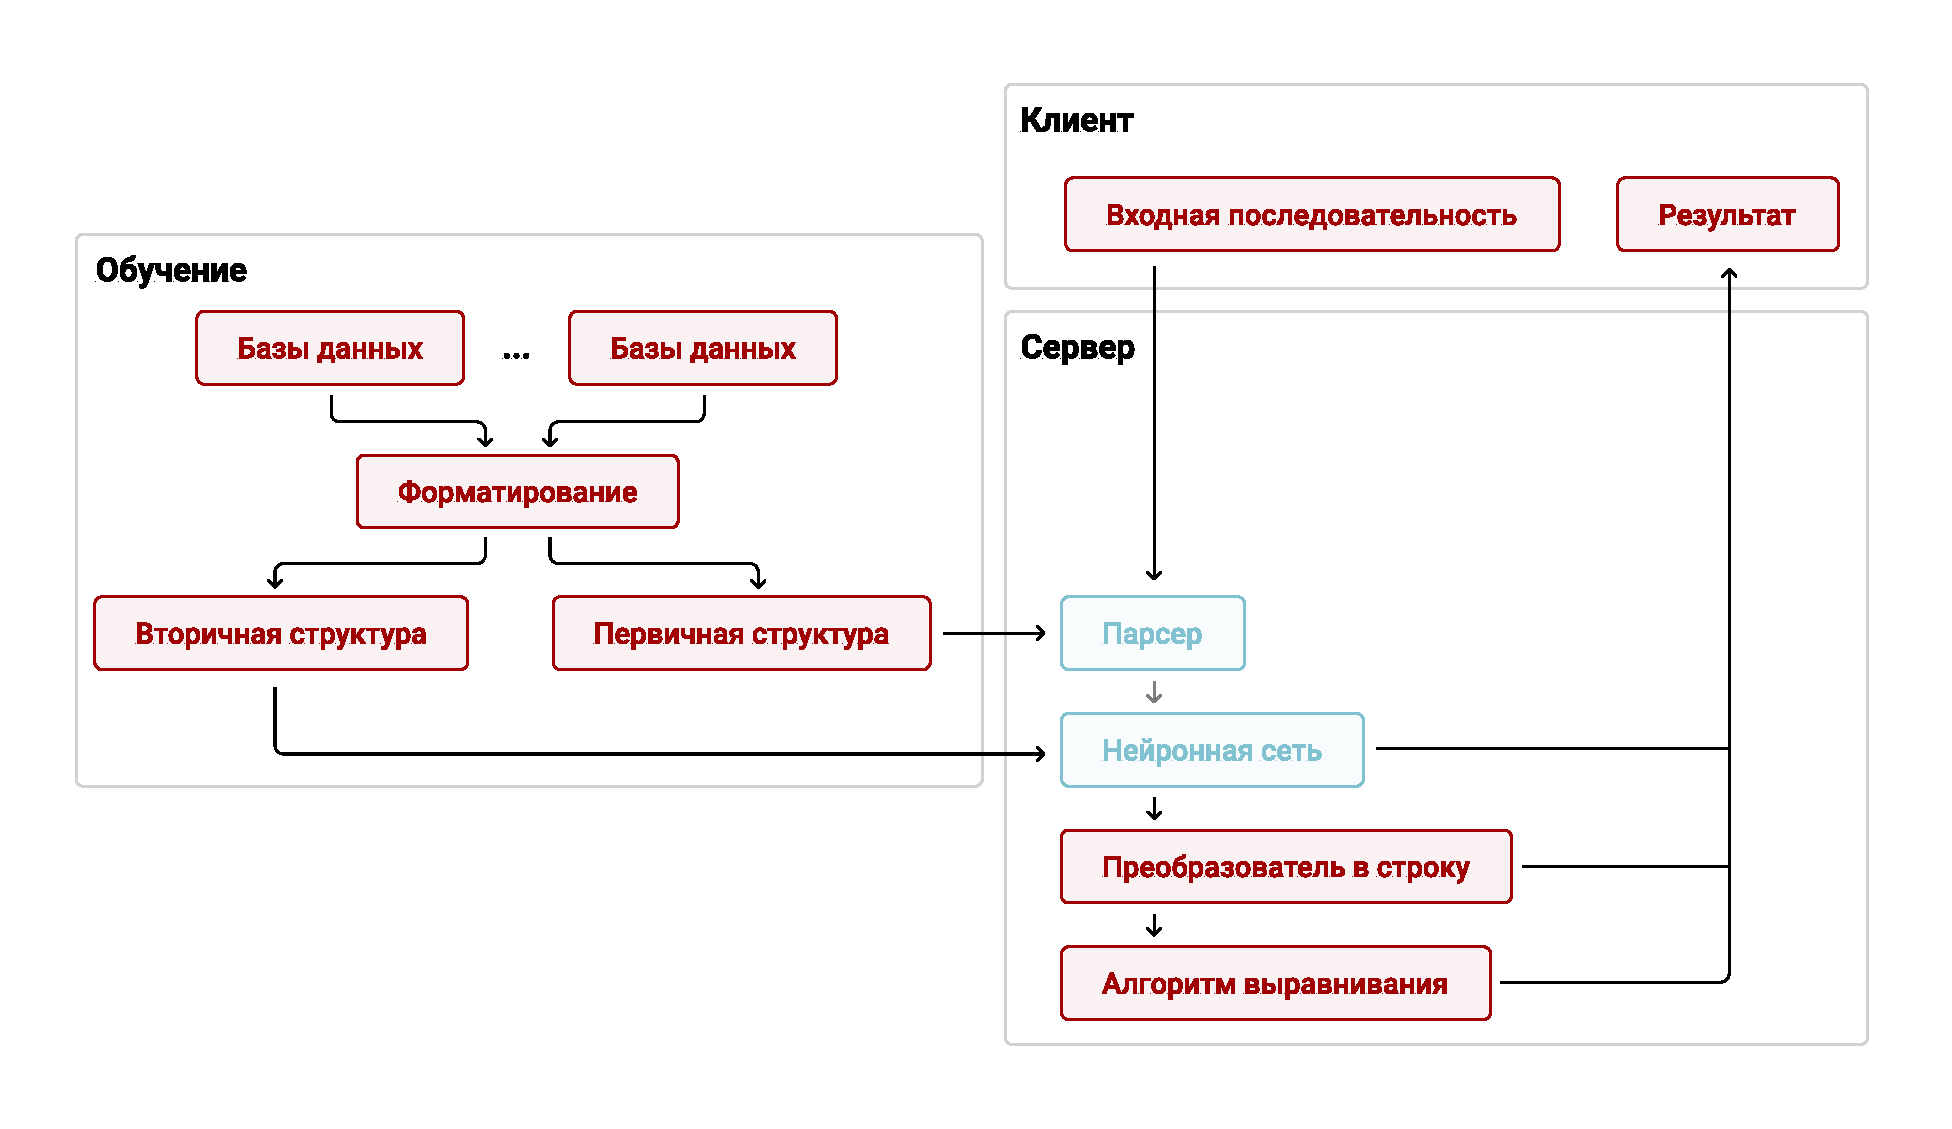
\includegraphics[width=12cm]{./pictures/diag3.pdf}
\end{frame}

\begin{frame}[fragile]
\transwipe[direction=90]
\frametitle{Подготовка данных}
\begin{tabular}{p{5cm} p{7cm}}
	\begin{itemize}
		\item Парсер --- распознает места возможных связей
		\item Нейросеть --- учится очищать результат работы парсера
		\item Представление данных в виде изображений
	\end{itemize} &
	\multirow{-3}*{\!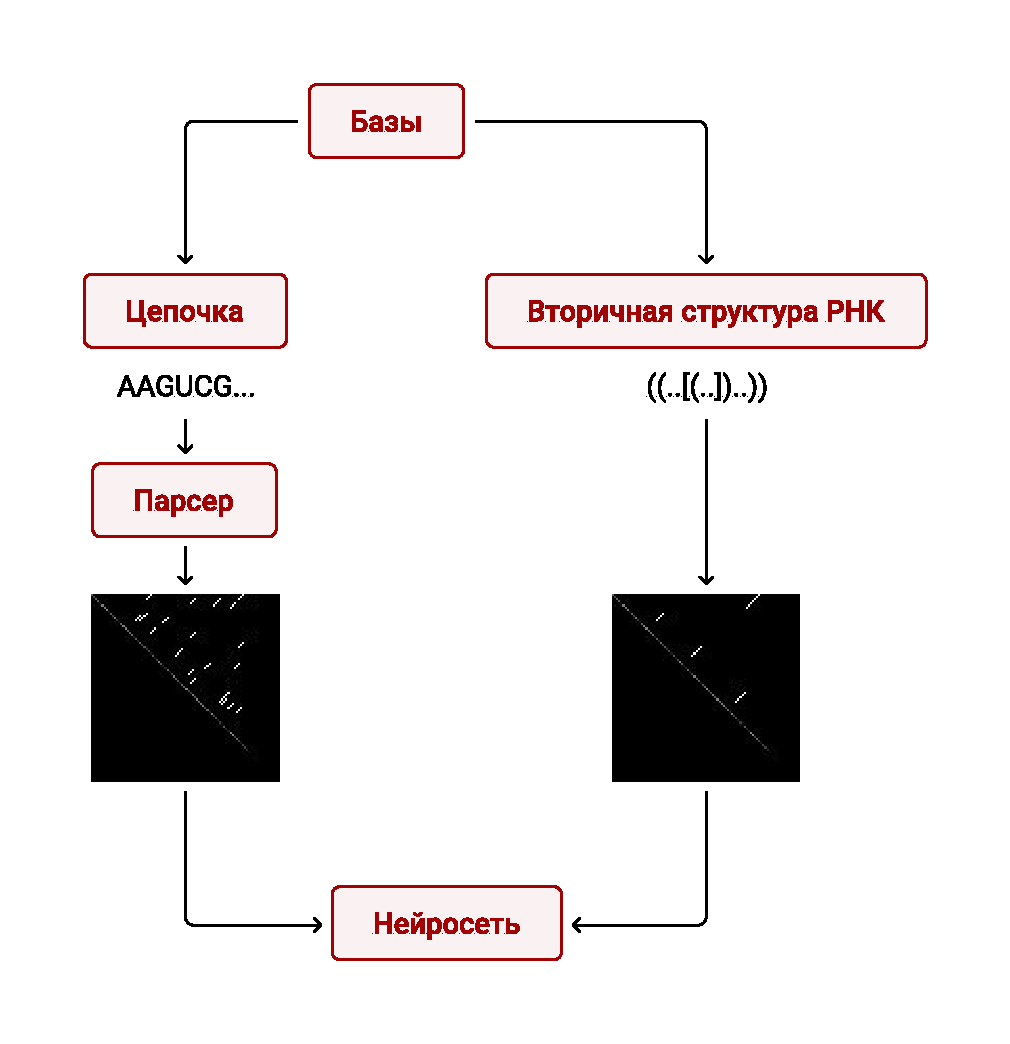
\includegraphics[width=7cm]{pictures/diag2.pdf}}\\
	\multirow{-1.75}*{\!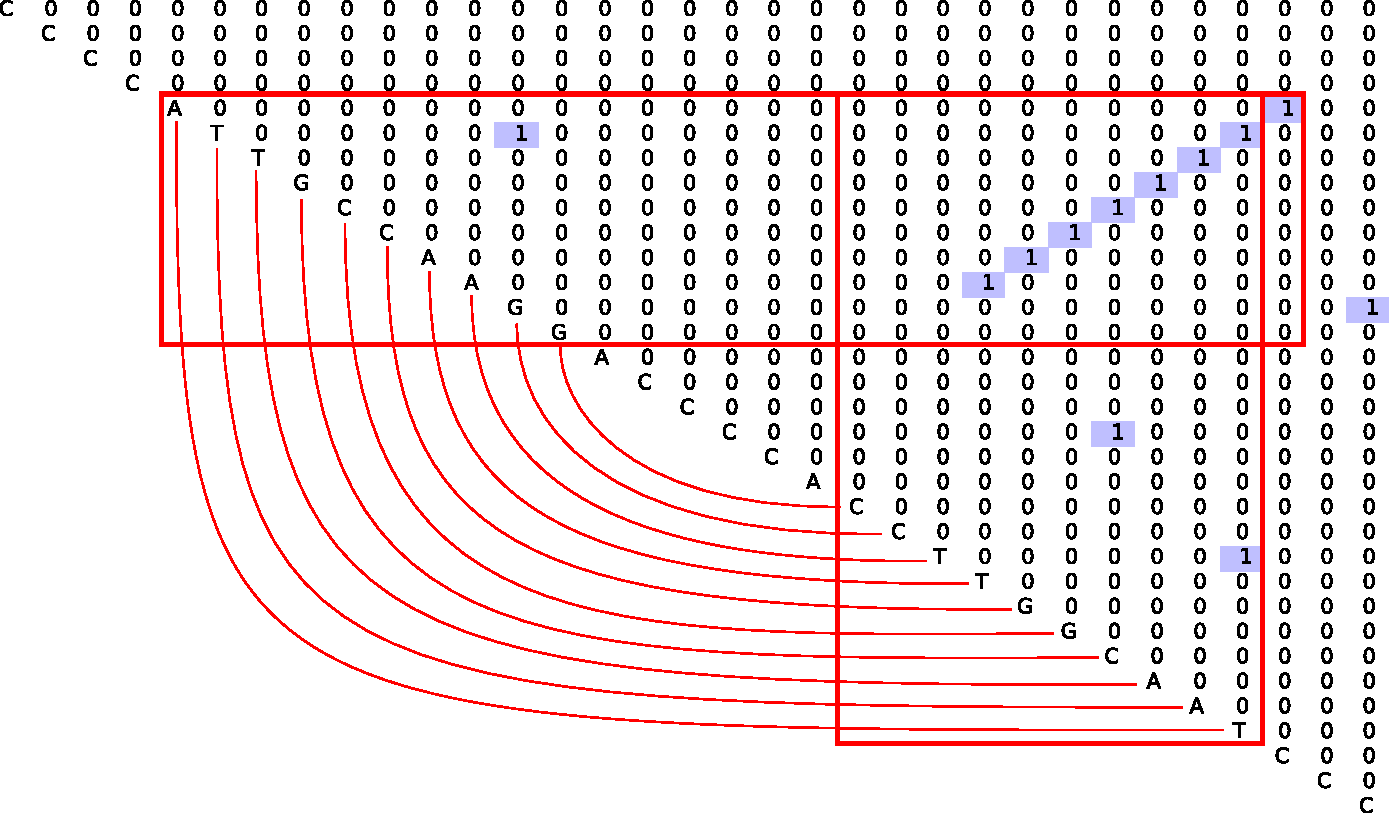
\includegraphics[width=4.5cm]{../pics/4.pdf}}
\end{tabular}

\end{frame}

\begin{frame}[fragile]
\transwipe[direction=90]
\frametitle{Архитектура конечного приложения}
\begin{tabular}{p{5cm} p{7cm}}
	\begin{itemize}
		\item Клиент-серверное приложение
		\item Пользователь может видеть промежуточные этапы работы системы
		\item Результат выраванивается, чтобы соответствовать биологическим законам
		
		
	\end{itemize} &
	%{\includegraphics[width=5cm]{../DNA_RNA_structure_(full).png}}
	\multirow{-2}*{\!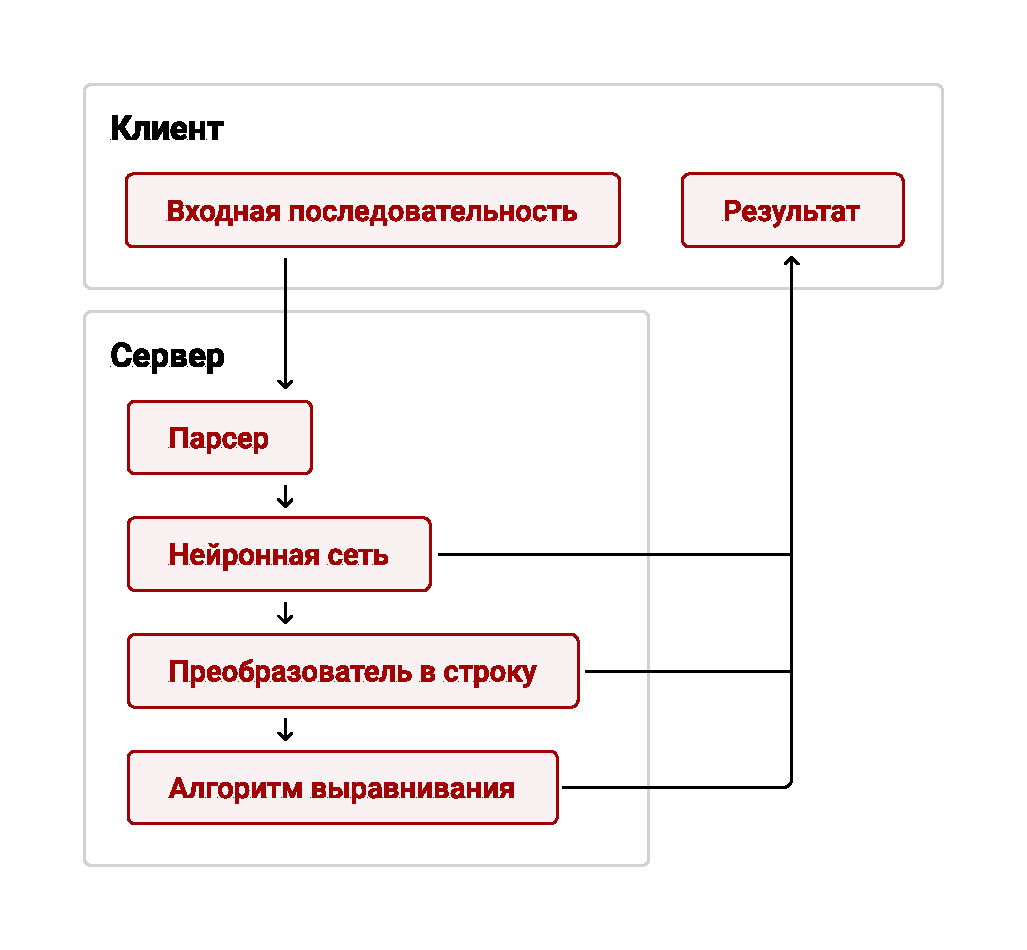
\includegraphics[width=7cm]{pictures/diag1.pdf}}
\end{tabular} \\ \bigskip 
Система доступна по адресу \url{http://www.secondarystructure.tk/}

\end{frame}

\begin{frame}
\transwipe[direction=90]
\frametitle{Используемые технологии}
\begin{itemize}
	\item Связь через \textit{REST API}
	\item Сервер --- \textit{Python3}, \textit{Flask}, \textit{Waitress}, \textit{Biopython}
	\item Клиент --- \textit{Bulma.io}, \textit{Vue.js}, \textit{axios}
	
\end{itemize}\medskip

\end{frame}
	


\begin{frame}
  \transwipe[direction=90]
  \frametitle{Результаты}
  \begin{itemize}
    \item Создан инструмент для обработки данных для обучения нейронной сети. Собраны, проанализированы и обработаны данные из нескольких источников --- \textit{RNA STRAND}, \textit{Pseudobase++}, \textit{RNACentral}
    \item Разработан алгоритм перевода полученных последовательностей в биологически возможные
    \item Разработано клиент-серверное приложение, позволяющее предсказывать вторичную структуру РНК последовательностей
    \item По результатам работы поданы тезисы на постерную секцию международной конференции BiATA 2020
  \end{itemize}

\end{frame}

\end{document}
